\subsubsection{Wave pool}
\label{sec.tests.wavepool}

In this one-dimensional test, we pass a short wavelength, linear wave through a static refined region.  The full domain is from 0 to 1 and the refined region is set from 0.25 to 0.75 at all times.  We modify the left boundary consistent with a single linear sound wave with density given by $\rho(x,t) = \rho_0 (1 + A \sin(kx - \omega t))$, where the amplitude is $A = 0.01$ and the wavelength $\lambda = k/2\pi = 0.1$, and similar expressions exist for the pressure and velocity.  The initial, unperturbed density and pressure are set to unity and we adopt $\gamma = 1.4$.  The (unrefined) root grid is covered with 100 cells, resulting in a wavelength for the linear wave of only 10 cells.  This is, therefore, a challenging problem for hydro methods.  We are particularly interested in any reflection or artifacts introduced by the wave entering and exiting the refined regions.

Figure~\ref{fig.wavepool} shows the evolution of the wave at three different times ($t = 0.2, 0.3$ and 0.8) for three of our solvers (PPM, Zeus, and MUSCL).  The leftmost column show the wave just before it enters the refined region so that we can gauge how the solver is operating in the absence of AMR, the center column shows the wave after it has fully entered the refined region, and the rightmost column shows the wave well after it has exited the refined region.

Beginning with the PPM, we see that even before it has entered the refine region, the wave is slightly damped, which is not unexpected for such a short wavelength mode, even for PPM.  The remaining panels demonstrate that the wave cleanly enters and exits the refined region.  No significant reflection is seen, either on entry or exit, and the amount of damping is mild.

For the Zeus solver, we see that even before it has entered the refined region, there are small oscillations excited behind the wave; although it is also worth noting that the wave itself is beautifully propagated without significant damping or phase errors.  In this test, we use only our standard, low amount of quadratic artificial viscosity -- these waves can be damped by additional viscosity, but we do not add any in order to be sensitive to any artifacts at the grid boundary.  The remaining panels show that the trailing oscillations continue, but do not generate any additional noise -- the end result is similar to the case without any refined region.

Finally, the MUSCL solver shows also shows a very clean entry and exit from the refined region without any oscillations, although (for the PLM reconstruction used here) the wave is spread more than with the other methods.

\begin{figure}
\begin{center}
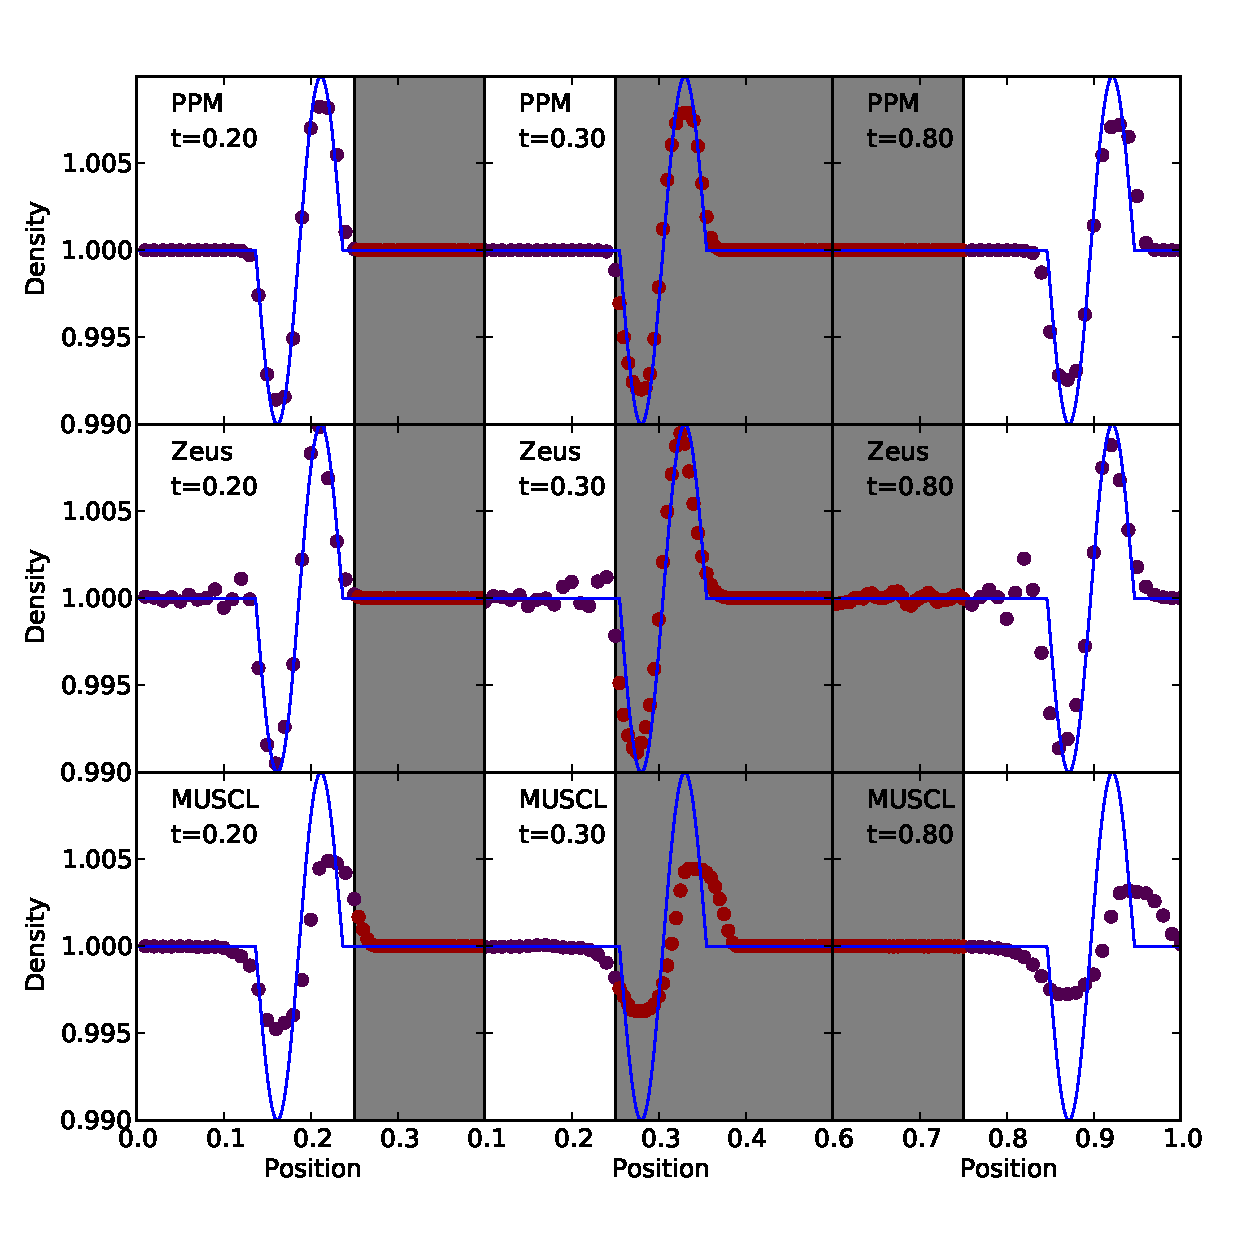
\includegraphics[width=0.8\textwidth]{figures/WavePool.eps}
\caption{This plot shows, for each column, three snap shots (at $t=0.2, 0.3$ and 0.8) of a linear wave as it propagates through the grid.  The static refined region extends from $x = 0.25$ to 0.75 and is shown in grey in each panel.  The individual cells are also color-coded by level: blue indicates the root grid, and red is for the refined region.  Each row shows the result for a different solver (top is PPM, middle is Zeus, and the bottom is MUSCL).   The solid line shows the analytic solution for a linear, undamped wave.  Note that we focus each panel on a small region of the entire domain to better show the wave itself.}
\label{fig.wavepool}
\end{center}
\end{figure}
